\documentclass{ltjsarticle}
% 数式
\usepackage{amsmath}
% 画像表示
\usepackage{graphicx}
\usepackage{svg}
% 表を使いやすく
\usepackage{tabularx}
% 図の場所を強制
\usepackage{here}
% URL
\usepackage{url}
% ハイパーリンクがつく
\usepackage{hyperref}
% 文章を枠で囲う
\usepackage{ascmac}
% enumerateのラベルを変更可能に
\usepackage{enumitem}
% 外部のファイルからテキストを読み込む
\usepackage{moreverb}
% ソースコードの表示用
\usepackage{listings}
%ソースコードの表示に関する設定
\lstset{
    basicstyle={\ttfamily},
    identifierstyle={\small},
    commentstyle={\smallitshape},
    keywordstyle={\small\bfseries},
    ndkeywordstyle={\small},
    stringstyle={\small\ttfamily},
    frame={tb},
    breaklines=true,
    columns=[l]{fullflexible},
    numbers=left,
    xrightmargin=0\zw,
    xleftmargin=3\zw,
    numberstyle={\scriptsize},
    stepnumber=1,
    numbersep=1\zw,
    lineskip=-0.5ex
}
\renewcommand{\lstlistingname}{リスト}
% 中央揃え(tabularx)
\newcolumntype{C}{>{\centering\arraybackslash}X}
% 左揃え(tabularx)
\newcolumntype{L}{>{\scriptsize\raggedright\arraybackslash}X}
% 右揃え(tabularx)
\newcolumntype{R}{>{\scriptsize\raggedleft\arraybackslash}X}
% 行の中心に配置
\newcommand{\CenterRow}[2]{
    \dimen0=\ht\strutbox%
    \advance\dimen0\dp\strutbox%
    \multiply\dimen0 by#1%
    \divide\dimen0 by2%
    \advance\dimen0 by-.5\normalbaselineskip%
    \raisebox{-\dimen0}[0pt][0pt]{#2}
}


\title{\vspace{-4cm}
制御工学実験Ⅱ テーマ:マイコン基礎応用
}
\author{
    制御情報システム工学科 4年 10番 國安柾希
}

\begin{document}
\maketitle

\subsection*{実施評価}
\begin{tabularx}{\textwidth}{|p{130mm}|C|C|} \hline
    \CenterRow{2}{評価項目} & 自己評価 & 担当評価 \\ \hline
    実験開始までに実験テキストや実験ノートを準備できており,事前課題がある場合は,それに取り組んでいた.
    & \CenterRow{2}{A} & \\ \hline
    担当者による指示をよく聞き,不注意による無用な誤りなく安全に実験を行うことができた.
    & \CenterRow{2}{A} & \\ \hline
    回路やプログラムを自分で作成し,グループワークの場合は自らの役割を全うするなど,課題に対して積極的に取り組むことができた.
    & \CenterRow{2}{A} & \\ \hline
    与えられた課題を時間内に達成し,結果を正確に記録または出力できた. \par
    & \CenterRow{2}{A} & \\ \hline
    使用器具の後片付けや実験場所の清掃をきちんと行った. \par
    & \CenterRow{2}{A} & \\ \hline
\end{tabularx}

\subsection*{レポート評価}
\begin{tabularx}{\textwidth}{|p{130mm}|C|C|} \hline
    \CenterRow{2}{評価項目} & 自己評価 & 担当評価 \\ \hline
    章立ては適切であり,それぞれの章における記載内容は自作のものである.引用がある場合は,その旨を明記している.
    & \CenterRow{2}{A} & \\ \hline
    図・表の書き方は裏面の要領に準じており,自作のものである.(担当者が許可しない限り,指導書の図すら引用してはいけない)
    & \CenterRow{2}{A} & \\ \hline
    使用器具や実験環境について,実験結果を再現するのに十分な情報を記載している. \par
    & \CenterRow{2}{A} & \\ \hline
    課題に関する計測結果や出力結果を整理して記載し,結果に対する独自の考察を述べている.
    & \CenterRow{2}{A} & \\ \hline
    研究課題に取り組み,適切な参考文献を基に答えを導き出している. \par
    & \CenterRow{2}{A} & \\ \hline
\end{tabularx}

\begin{center}
    \begin{tabularx}{100mm}{|C|C|C|} \hline
        実施点\par(50) & レポート点\par(50) & 合計点\par(100) \\ \hline
        \ \par\ \par & & \\ \hline
    \end{tabularx}
\end{center}

\newpage
\section{実験目的}

今までの実験では,PCで作成したプログラムをArduinoに書き込んで実行してきた.しかし,Arduinoへの書き込みのみでは,要求する動作が複数ある場合,選択することが困難になる場合がある.
それを解決するために,今回の実験では,Arduinoのプログラムを書き込んだ後にArduinoとPC間でシリアル通信を行って,PCからコマンドを送信してハードウエアの制御を行う.
また,Webサイトから必要な情報を収集し実際に実装することで,具体的な知識やスキルを身に着け,そのシステム構築を通して,PCとArduinoの連携を利用した,より複雑なシステムの構築方法を身に着ける.

% タイトルは自分で考える
% 「実験目的」で出したキーワードについて,数式やフローチャート,図や表を利用して詳細な仕組みを説明する.

\section{構築した組み込みシステム}
\subsection{実験課題}
以下の条件を満たすシステムを構築する
% 半固定抵抗のつまみの角度(位置)に対応してサーボモータの
% 角度を変える(自動車のパワーステアリングのイメージ)
\begin{itemize}
    \item 入力:シリアル通信(Rx),半固定抵抗(10kΩ)
    \item 出力:シリアル通信(Tx),赤黄LEDを各1個,サーボモータ
    \item 動作:\begin{enumerate}
        \item PCからコマンド操作(シリアルモニタから文字列を送信して操作)

        “r,ooo”: 赤色LEDをoooの明るさにする(oooは0-255の整数)

        “y,ooo”: 黄色LEDをoooの明るさにする 

        “w,ooo,OOO”: 赤色LEDをooo,黄色LEDをOOOの明るさにする 

        “s”: 赤色LEDと黄色LEDの現在の明るさをPCに送る
        \item 半固定抵抗のつまみの角度(位置)に対応してサーボモータの角度を変える(自動車のパワーステアリングのイメージ)
    \end{enumerate}
\end{itemize}

\subsection{実験結果}
作成したシステムの実際の回路,回路図を図\ref{fig:task1},プログラムをリスト\ref{lst:task1prog}に示す.\\\\
\begin{figure}[h]
  \centering
  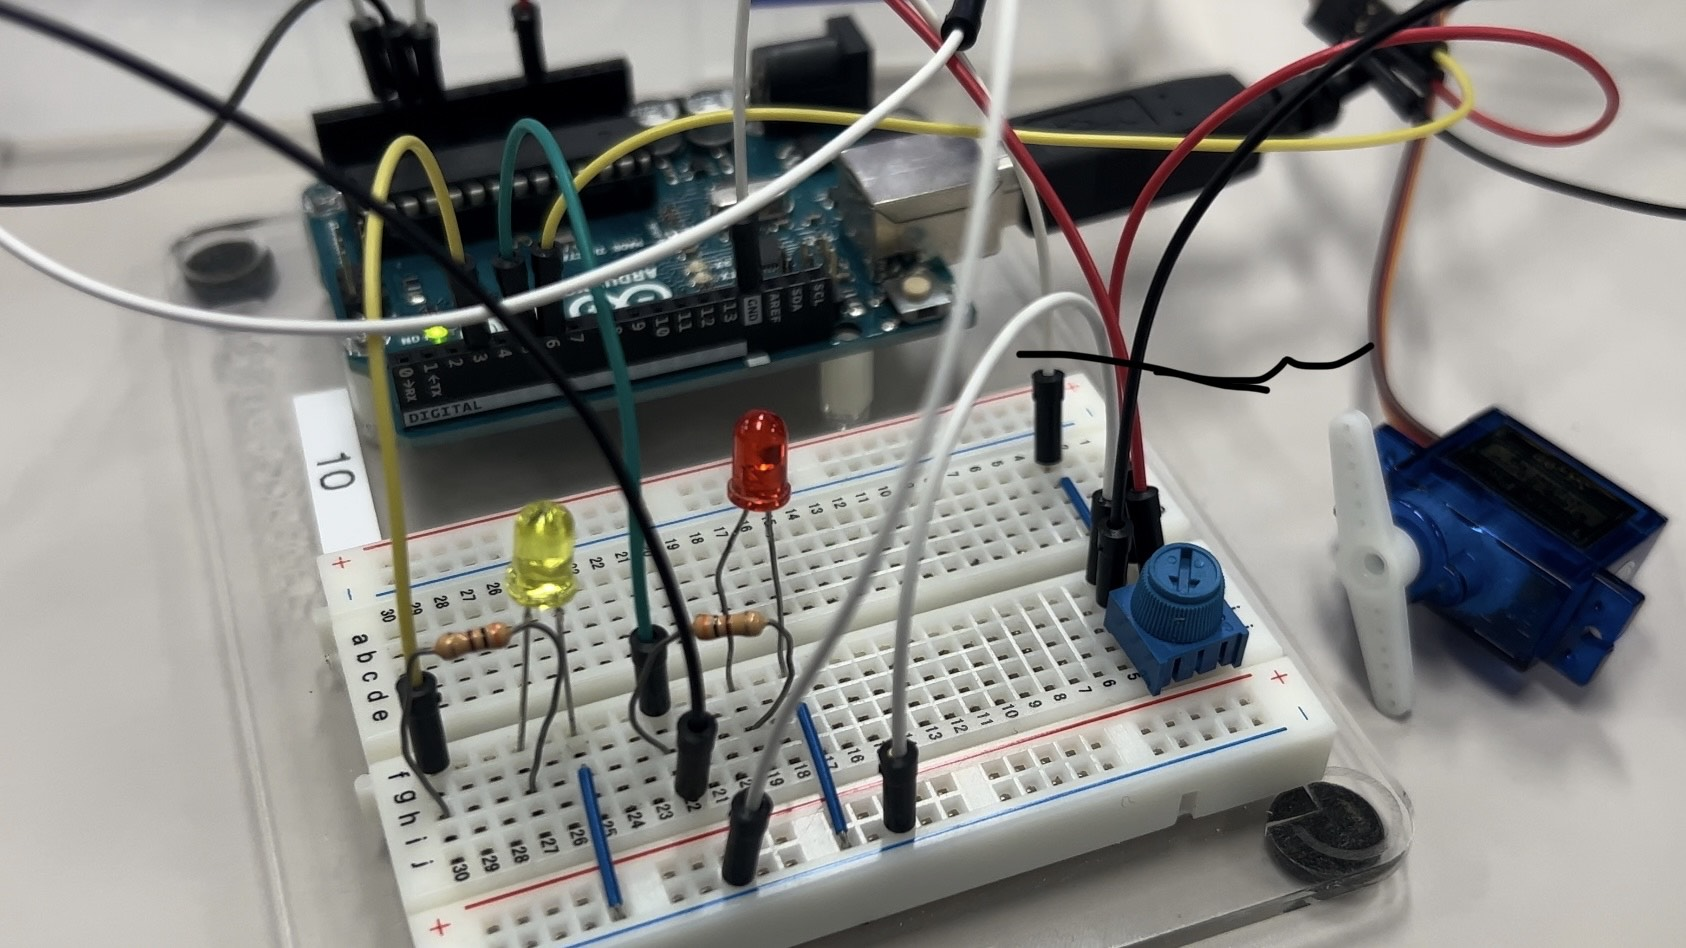
\includegraphics[width=\linewidth]{figures/task1.jpg}
  \caption{実際の回路}
  \label{fig:task1}
\end{figure}

\clearpage

\lstinputlisting[caption=課題のプログラム,label=lst:task1prog]{src/task0607.ino}


\section{考察}




\section{感想}

\begin{thebibliography}{9}
    % \bibitem{key} title, hostname, \url{url}, (参照日 YYYY年 MM月 DD日)
\end{thebibliography}
\end{document}
